\section{WebApp}
A web application is a computer program that utilizes web browsers and web technology to perform tasks over the Internet.\\

Web applications use a combination of server-side scripts (PHP and ASP) to handle the storage and retrieval of the information, and client-side scripts (JavaScript and HTML) to present information to users. This allows users to interact with the company using online forms, content management systems, shopping carts and more. In addition, the applications allow employees to create documents, share information, collaborate on projects, and work on common documents regardless of location or device.\\

\subsection{How it works? }
Web applications are usually coded in browser-supported language such as JavaScript and HTML as these languages rely on the browser to render the program executable. Some of the applications are dynamic, requiring server-side processing. Others are completely static with no processing required at the server.\\

The web application requires a web server to manage requests from the client, an application server to perform the tasks requested, and, sometimes, a database to store the information. Application server technology ranges from ASP.NET, ASP and ColdFusion, to PHP and JSP.\\
Here's what a typical web application flow looks like:\\


\begin{itemize}
  \item User triggers a request to the web server over the Internet, either through a web browser or the application’s user interface

  \item Web server forwards this request to the appropriate web application server
  \item Web application server performs the requested task – such as querying the database or processing the data – then generates the results of the requested data
  \item Web application server sends results to the web server with the requested information or processed data

  \item Web server responds back to the client with the requested information that then appears on the user’s display
\end{itemize}\\

\subsection{Let's Create our App} 
The technology we will use to build out web app is React app it's very fast and very scalable web framework managed and developed by Facebook. and once it got loaded then everythin is stored and work easily.\\

Here is the final link of Web App : - \url{https://watermonitoring.netlify.app/}\\

To make web app more interactive and knowledgeable we include some best pond animation and Facts about water\\

Now Lets talk about Code We Will only talk about main code not about animation as it's very difficult to understand those animations so we will first directly jump into the Main code and in last animation code (optional*) \\

This is the main App.js Code which is starting point of our app\\

\begin{lstlisting}[language=javascript, caption={Water Monitoring App}]

import React from 'react';
import './App.css';
import * as tf from "@tensorflow/tfjs"
import Homepage from './Components/Homepage';

function App() {
  return (
    <div id="canvas-wrap">
      <canvas id="canvas"></canvas>
      <div id="overlay">
        <Homepage/>
      </div>
    </div>
  );
}
export default App;

\end{lstlisting}\\

Here is the main Homepage which include graphs between effect on Temperature and D.O and the effect of pH on D.O, Prediction input and facts \\

\begin{lstlisting}[language=javascript, caption={Homepage of ML app}]

import React, { useState } from 'react';
import * as tf from "@tensorflow/tfjs"
import { Scatter } from 'react-chartjs-2';
import d from "../data/water.json"
import facts from "../data/facts.json"


const modelUrl = "https://raw.githubusercontent.com/tarun-29/Water-Project-Intern/master/tfjs/model.json"
const model = async (temp, ph, setAns) => {
    console.log("hello babes")
    return await tf.loadLayersModel(modelUrl).then(m => {
        if (parseFloat(temp) && parseFloat(ph)) {
            if (temp === 0 || ph === 0) {
                alert("Please enter valid values")
                return
            }
            else {
                var dat = [parseFloat(temp), parseFloat(ph)]
                var shap = [1, 2]
                var results = m.predict(tf.tensor2d(dat, shap));
                //  console.log(results.dataSync())
                Promise.resolve(results.dataSync()).then(s => {
                    setAns(s)
                })
            }
        }
        else{
            alert("Enter numeric value")
            return
        }

    })
}

const tempArray= []
tempArray.push(d.map(m=>{
    var obj = {}
    obj["y"] = m.DO
    obj["x"] = m.Temp
    return obj
}))

const pHArray= []
pHArray.push(d.map(m=>{
    var obj = {}
    obj["y"] = m.DO
    obj["x"] = m.PH
    return obj
}))

const options = {
    legend: {
        labels: {
            fontColor: "white",
            fontSize: 18
        }
    },
    responsive: true,
    title: {
        display: true,
        fontColor: "white",
        fontSize: 15,
    },
    // tooltips: {
    //     mode: 'label',
    // },
    hover: {
        mode: 'nearest',
        intersect: true
    },
    scales: {
        xAxes: [{
            ticks: {
                fontColor: "white",
                fontSize: 15,
            },
            display: true,
            gridLines: {
                display: false,
            },
            scaleLabel: {
                display: true,
                labelString: 'Temperature',
                fontColor: "white",
                fontSize: 15
            }
        }],
        yAxes: [{
            ticks: {
                fontColor: "white",
                fontSize: 15,
            },
            display: true,
            gridLines: {
                display: false,
            },
            scaleLabel: {
                display: true,
                labelString: 'D.O(mg/L)',
                fontColor: "white",
                fontSize: 15
            }
        }]
    }
}

const options1 = {
    legend: {
        labels: {
            fontColor: "white",
            fontSize: 18
        }
    },
    responsive: true,
    title: {
        display: true,
        fontColor: "white",
        fontSize: 15,
    },
    // tooltips: {
    //     mode: 'label',
    // },
    hover: {
        mode: 'nearest',
        intersect: true
    },
    scales: {
        xAxes: [{
            ticks: {
                fontColor: "white",
                fontSize: 15,
            },
            display: true,
            gridLines: {
                display: false,
            },
            scaleLabel: {
                display: true,
                labelString: 'PH',
                fontColor: "white",
                fontSize: 15
            }
        }],
        yAxes: [{
            ticks: {
                fontColor: "white",
                fontSize: 15,
            },
            display: true,
            gridLines: {
                display: false,
            },
            scaleLabel: {
                display: true,
                labelString: 'D.O(mg/L)',
                fontColor: "white",
                fontSize: 15
            }
        }]
    }
}


const data1 = tempArray[0]
const data2 = pHArray[0]

const Temp = {
    labels: ['Scatter'],
    datasets: [
        {
            label: 'Temp vs D.O(mg/L)',
            fill: false,
            backgroundColor: 'rgba(75,192,192,0.4)',
            pointBorderColor: 'yellow',
            pointBackgroundColor: '#fff',
            pointBorderWidth: 1,
            pointHoverRadius: 5,
            pointHoverBackgroundColor: 'rgba(75,192,192,1)',
            pointHoverBorderColor: 'rgba(220,220,220,1)',
            pointHoverBorderWidth: 2,
            pointRadius: 2,
            pointHitRadius: 10,
            data: data1
        }
    ]
};

const ph = {
    labels: ['Scatter'],
    datasets: [
        {
            label: 'pH vs D.O(mg/L)',
            fill: false,
            backgroundColor: 'rgba(75,192,192,0.4)',
            // pointBorderColor: 'rgba(75,192,192,1)',
            pointBorderColor: 'yellow',
            pointBackgroundColor: '#fff',
            pointBorderWidth: 1,
            pointHoverRadius: 5,
            pointHoverBackgroundColor: 'rgba(75,192,192,1)',
            pointHoverBorderColor: 'rgba(220,220,220,1)',
            pointHoverBorderWidth: 2,
            pointRadius: 2,
            pointHitRadius: 10,
            data: data2
        }
    ]
};

function Homepage() {
    console.log(pHArray)
    const [count, setCount] = useState(0);
    const [temp, setTemp] = useState(0);
    const [PH, setPH] = useState(0);
    const [ans, setAns] = useState(0);
    return (
        <div style={{ color: "white", textAlign: 'center', fontSize: 25 }}>Water Quality Model
            <div style={{ display: "flex", flexDirection: 'row', justifyContent: "space-around" }} className="container">
                <div>
                    <div style={{ display: "flex", flexDirection: 'column', justifyContent: "space-around" }}>
                        <div >
                            <Scatter data={Temp} options={options} height={300} width={400} />
                        </div>
                        <div >
                            <Scatter data={ph} options={options1} height={300} width={400} />
                        </div>
                    </div>
                </div>
                <div style={{ display: "flex", flexDirection: 'column', justifyContent: "space-between" }}>

                    <div style={{ marginTop: 20 }} className="card-form">
                        <form className="signup">
                            <div className="form-title">Predictions of D.O(mg/L)</div>
                            <div className="form-body">
                                <div className="row">
                                    <input onChange={(e) => setTemp(e.target.value)} type="text" placeholder="Water Temp (20-30)" />
                                </div>
                                <div className="row">
                                    <input onChange={(e) => setPH(e.target.value)} type="text" placeholder="Water pH" />
                                </div>
                            </div>
                            <div className="rule"></div>
                            <div className="form-footer" style={{ display: "flex", flexDirection: 'row' }}>
                                <a href="/#" onClick={async () => { console.log(await model(temp, PH, setAns)) }}>Calculate<span className="fa fa-ban"></span></a>
                                <div style={{ color: 'black' }}>{parseFloat(ans).toFixed(4)}</div>
                            </div>
                        </form>
                    </div>
                    {(facts.length <= 100) ? (<div className="card">
                        <div id="circle"></div>
                        <h2>Facts</h2>
                        <p>{facts[count].Fact}</p>
                        <div className="content">
                            <a onClick={(e) => setCount(count + ((Math.floor(Math.random() * 100))) - count)}>New Fact</a>
                        </div>
                    </div>) : (<div>No Fact</div>)}
                </div>
            </div>
        </div>
    );
}

export default Homepage;

\end{lstlisting}\\

\begin{lstlisting}[language=javascript, caption={Background animation}]
(function () {
      'use strict';
      window.addEventListener('load', function () {
        var canvas = document.getElementById('canvas');

        if (!canvas || !canvas.getContext) {
          return false;
        }

        /********************
          Random Number
        ********************/

        function rand(min, max) {
          return Math.floor(Math.random() * (max - min + 1) + min);
        }

        /********************
          Var
        ********************/

        // canvas 
        var ctx = canvas.getContext('2d');
        var X = canvas.width = window.innerWidth;
        var Y = canvas.height = window.innerHeight;
        var mouseX = null;
        var mouseY = null;

        /********************
          Animation
        ********************/

        window.requestAnimationFrame =
          window.requestAnimationFrame ||
          window.mozRequestAnimationFrame ||
          window.webkitRequestAnimationFrame ||
          window.msRequestAnimationFrame ||
          function (cb) {
            setTimeout(cb, 17);
          };

        /********************
          Wave
        ********************/
        var waves = [];

        function Wave(ctx, x, y, r) {
          this.ctx = ctx;
          this.init(x, y, r);
        }

        Wave.prototype.init = function (x, y, r) {
          this.x = x;
          this.y = y;
          this.r = r;
          this.l = rand(100, 150);
        };

        Wave.prototype.draw = function () {
          ctx = this.ctx;
          ctx.save();
          ctx.beginPath();
          ctx.strokeStyle = 'rgb(149, 188, 249)';
          ctx.arc(this.x, this.y, this.r, 0, Math.PI * 2, false);
          ctx.stroke();
          ctx.restore();
        };

        Wave.prototype.updateParams = function () {
          this.r += 1;
        };

        Wave.prototype.deleteWave = function (i) {
          if (this.r > this.l) {
            waves.splice(i, 1);
          }
        };

        Wave.prototype.render = function (i) {
          this.updateParams();
          this.deleteWave(i);
          this.draw();
        };

        /********************
          Fish
        ********************/

        var fishes = [];
        var fishDir = [true, false];
        var fishColors = ['255, 111, 147', '49, 194, 243', '255, 158, 0', '107, 136, 255'];

        function Fish(ctx, x, y, r, d, c) {
          this.ctx = ctx;
          this.init(x, y, r, d, c);
        }

        Fish.prototype.init = function (x, y, r, d, c) {
          this.d = d;
          this.x = x;
          this.y = y;
          this.r = r;
          this.c = c;
          this.rad = this.a * Math.PI / 180;
          if (this.d === true) {
            this.v = {
              x: rand(1, 2) * 0.5,
              y: rand(-1, 1) * 0.5
            };
          } else {
            this.v = {
              x: rand(-2, -1) * 0.5,
              y: rand(-1, 1) * 0.5
            };
          }
        };

        Fish.prototype.draw = function () {
          ctx = this.ctx;
          ctx.save();
          ctx.beginPath();
          ctx.fillStyle = 'rgb(' + this.c + ')';
          ctx.scale(2, 1);
          ctx.arc(this.x / 2, this.y, this.r, 0, Math.PI * 2, false);
          ctx.fill();
          ctx.beginPath();
          if (this.d === true) {
            ctx.moveTo(this.x / 2 + this.r / 2, this.y);
            ctx.lineTo(this.x / 2 + this.r + this.r / 2, this.y + this.r / 2);
            ctx.lineTo(this.x / 2 + this.r + this.r / 2, this.y - this.r / 2);
          } else {
            ctx.moveTo(this.x / 2 - this.r / 2, this.y);
            ctx.lineTo(this.x / 2 - this.r - this.r / 2, this.y + this.r / 2);
            ctx.lineTo(this.x / 2 - this.r - this.r / 2, this.y - this.r / 2);
          }
          ctx.fill();
          ctx.restore();
        };

        Fish.prototype.updatePosition = function () {
          this.x -= this.v.x;
          this.y += this.v.y;
        };

        Fish.prototype.wrapPosition = function () {
          if (this.x + this.r + this.r > X) {
            this.v.x *= -1;
            this.d = true;
          }
          if (this.x - this.r - this.r < 0) {
            this.v.x *= -1;
            this.d = false;
          }
          if (this.y + this.r > Y) {
            this.v.y *= -1;
          }
          if (this.y - this.r < 0) {
            this.v.y *= -1;
          }
        };

        Fish.prototype.resize = function () {
          this.x = rand(0, X);
          this.y = rand(0, Y);
        };

        Fish.prototype.render = function () {
          this.updatePosition();
          this.wrapPosition();
          this.draw();
        };

        /********************
          Grass
        ********************/

        // var
        var grassNum = 200;
        var grasses = [];

        function Grass(ctx, x, y, w, t) {
          this.ctx = ctx;
          this.init(x, y, w, t);
        }

        Grass.prototype.init = function (x, y, w, t) {
          this.x = x;
          this.y = y;
          this.w = w;
          this.t = t;
          this.a = 0;
          this.rad = this.a * Math.PI / 180;
          this.c = '255, 255, 255';
          this.v = {
            x: Math.cos(this.rad),
            y: Math.sin(this.rad)
          };
          this.xt = this.x + this.w;
          this.yt = this.y - this.t;
          this.xb = this.x + this.w + this.w;
        };

        Grass.prototype.updateParams = function () {
          this.a += Math.random();
          this.rad = this.a * Math.PI / 180;
          this.v.x = Math.cos(this.rad) * 0.3;
          this.v.y = Math.sin(this.rad) * 0.3;
        };

        Grass.prototype.updatePosition = function () {
          this.xt += this.v.x;
        };

        Grass.prototype.draw = function () {
          ctx = this.ctx;
          ctx.save();
          ctx.fillStyle = 'rgb(86, 116, 25)';
          ctx.beginPath();
          ctx.moveTo(this.x, this.y);
          ctx.lineTo(this.xt, this.yt);
          ctx.lineTo(this.xb, this.y);
          ctx.closePath();
          ctx.fill();
          ctx.restore();
        };

        Grass.prototype.resize = function () {
          for (var i = 0; i < grassNum; i++) {
            grasses[i].init(rand(-10, X + 10), Y, rand(2.5, 5), rand(100, 200));
          }
        };

        Grass.prototype.render = function () {
          this.updateParams();
          this.updatePosition();
          this.draw();
        };

        for (var i = 0; i < grassNum; i++) {
          var grass = new Grass(ctx, rand(-10, X + 10), Y, rand(2.5, 5), rand(100, 200));
          grasses.push(grass);
        }

        /********************
          Bubble
        ********************/

        // var
        var bubbleNum = 30;
        var bubbles = [];

        function Bubble(ctx, x, y, r) {
          this.ctx = ctx;
          this.init(x, y, r);
        }

        Bubble.prototype.init = function (x, y, r) {
          this.x = x;
          this.y = y;
          this.r = r;
          this.a = rand(1, 10);
          this.dist = rand(1, 10);
          this.rad = this.a * Math.PI / 180;
          this.c = '255, 255, 255';
          this.v = {
            x: Math.sin(this.rad),
            y: Math.cos(this.rad)
          };
        };

        Bubble.prototype.updateParams = function () {
          this.a += 1;
          this.rad = this.a * Math.PI / 180;
          this.y -= 1;
        };

        Bubble.prototype.wrapPosition = function () {
          if (this.x - this.r > X) {
            this.x = 0;
          }
          if (this.x + this.r < 0) {
            this.x = X;
          }
          if (this.y - this.r > Y) {
            this.y = 0;
          }
          if (this.y + this.r < 0) {
            this.y = Y;
          }
        };

        Bubble.prototype.draw = function () {
          ctx = this.ctx;
          ctx.save();
          ctx.beginPath();
          ctx.globalAlpha = 0.3;
          ctx.fillStyle = 'rgb(255, 255, 255)';
          ctx.arc(Math.cos(this.rad) * this.dist + this.x, Math.sin(this.rad) * this.dist + this.y, this.r, Math.PI * 2, false);
          ctx.fill();
          ctx.closePath();
          ctx.restore();
        };

        Bubble.prototype.resize = function () {
          this.x = rand(0, X);
          this.y = rand(0, Y);
        };

        Bubble.prototype.render = function () {
          this.updateParams();
          this.wrapPosition();
          this.draw();
        };

        for (var i = 0; i < bubbleNum; i++) {
          var bubble = new Bubble(ctx, rand(0, X), rand(0, Y), rand(1, 10));
          bubbles.push(bubble);
        }

        /********************
          Render
        ********************/

        function render() {
          ctx.clearRect(0, 0, X, Y);
          for (var i = 0; i < grasses.length; i++) {
            grasses[i].render();
          }
          for (var i = 0; i < bubbles.length; i++) {
            bubbles[i].render();
          }
          for (var i = 0; i < fishes.length; i++) {
            fishes[i].render();
          }
          for (var i = 0; i < waves.length; i++) {
            waves[i].render(i);
          }
          requestAnimationFrame(render);
        }

        render();

        /********************
          Event
        ********************/

        // resize
        function onResize() {
          X = canvas.width = window.innerWidth;
          Y = canvas.height = window.innerHeight;
          for (var i = 0; i < grasses.length; i++) {
            grasses[i].resize();
          }
          for (var i = 0; i < bubbles.length; i++) {
            bubbles[i].resize();
          }
        }

        window.addEventListener('resize', function () {
          onResize();
        });

        canvas.addEventListener('click', function (e) {
          mouseX = e.clientX;
          mouseY = e.clientY;
          var fish = new Fish(ctx, mouseX, mouseY, rand(5, 15), fishDir[rand(0, 1)], fishColors[rand(0, fishColors.length - 1)]);
          fishes.push(fish);
          var wave = new Wave(ctx, mouseX, mouseY, 0);
          waves.push(wave);
        }, false);

      });
    })();
\end{lstlisting}

\subsection{Chart.js}
The chart which are plotted in website are done using the best node package manager graph.js and it's very usable the installation command of the library is shown below


\begin{lstlisting}[language=bash, caption={Installation command graph.js}]
npm install chart.js --save
\end{lstlisting}

Here Our Web App portion is done one interesting point about this web app is that it only require Internet while loading the page once that's it when you make any prediction using this web app then it will predict using making any request to API or over cloud that's the main and very important point of this app. It's only needed to be load once and use anytime anywhere you want without internet(No Backend) (Condition you have to make data by Your self don't fetch from cloud)\\


\includegraphics[width=0.8\textwidth]{images/react.png}\\

\section{Mobile App React Native} 

\subsection{Introduction}

\begin{itemize}
  \item Create native apps for Android and iOS using React :- React Native combines the best parts of native development with React, a best-in-class JavaScript library for building user interfaces.\\
  Use a little—or a lot. You can use React Native today in your existing Android and iOS projects or you can create a whole new app from scratch.
  \item Written in JavaScript—rendered with native code :- React primitives render to native platform UI, meaning your app uses the same native platform APIs other apps do.\\
Many platforms, one React. Create platform-specific versions of components so a single codebase can share code across platforms. With React Native, one team can maintain two platforms and share a common technology—React.
  \item Native Development For Everyone:- React Native lets you create truly native apps and doesn't compromise your users' experiences. It provides a core set of platform agnostic native components like View, Text, and Image that map directly to the platform’s native UI building blocks.
  \item Seamless Cross-Platform :- React components wrap existing native code and interact with native APIs via React’s declarative UI paradigm and JavaScript. This enables native app development for whole new teams of developers, and can let existing native teams work much faster.
  
\end{itemize}

\subsection{Let's Jump to Code}
Let's understand the code behind very simple yet complex machine learning app as the backend api are already completed in chapter 3 not it's time to use that api in react native app the react native app is very different from react app because in web app we didn't use the api to make prediction as tensorflow already included in web app but mobile application are light so we have to make calculation on cloud because it can't perform high computation in mobile phone. So let's get in\\


\includegraphics[width=0.8\textwidth]{images/fish.png}\\

\begin{lstlisting}[language=javascript, caption={Mobile App Water Monitoring}]

import React, { useState } from 'react';
import { StyleSheet, Text, View, TouchableWithoutFeedback, Keyboard, Image, ActivityIndicator } from 'react-native';
import { Input, Button } from 'react-native-elements';
import axios from "axios"

const model = async (temp, ph, setAns) => {
  console.log("temp, ph")
  console.log(temp, ph)
  var url = `https://watertensorflow.herokuapp.com/${temp}/${ph}`
  axios.get(url).then(data => {
    console.log(data.data.ans)
    setAns(data.data.ans)
  })
}

const fetchData = async (setTemp, setPh, setAns, t, p, setActivity) => {
  setActivity(1)
  const temp = "https://api.thingspeak.com/channels/1171829/fields/1.json?api_key=EQMSTCUEFF2GMM76&results=2"
  const ph = "https://api.thingspeak.com/channels/1171829/fields/2.json?api_key=EQMSTCUEFF2GMM76&results=2"
  var getTemp = await axios.get(temp)
  var getPH = await axios.get(ph)
  getTemp.data.feeds.forEach(data => {
    if (data.field1 !== null) {
      setTemp(data.field1)
      t = data.field1
    }
  })
  getPH.data.feeds.forEach(data => {
    if (data.field2 !== null) {
      setPh(data.field2)
      p = data.field2
    }
  })
  await model(t, p, setAns)
  setActivity(0)
}

const staticData = async (t, p, setAns,setActivity) => {
  setActivity(1)
  console.log(typeof (t))
  if (parseFloat(t) <= 0 || parseFloat(p) <= 0) {
    alert("Please enter valid Temp and Ph")
    setAns(0)
    return
  }
  else {
    setTimeout(()=>{}, 3000)
    console.log("hello ji")
    await model(t, p, setAns)
    setActivity(0)
  }
}

export default function App() {
  const [temp, setTemp] = useState(0);
  const [Ph, setPh] = useState(0);
  const [tempStatic, setTempStatic] = useState(0);
  const [PhStatic, setPhStatic] = useState(0);
  const [ans, setAns] = useState(0);
  const [activity, setActivity] = useState(0);
  return (
    activity === 0 ?
      <TouchableWithoutFeedback onPress={Keyboard.dismiss} accessible={false}>
        <View style={styles.container}>
          <Image
            source={require("./assets/fish.png")}
            style={{ height: 150, width: 150 }}
          />
          <Text style={{ fontSize: 30, color: 'white', paddingBottom: 20 }}>Water Monitoring</Text>
          <View style={{ display: 'flex', flexDirection: 'row', paddingBottom: 20 }}>
            <Text style={{ fontSize: 20, color: 'white', paddingRight: 10 }}>Temp:  {temp}</Text>
            <Text style={{ fontSize: 20, color: 'white' }}>PH:  {Ph}</Text>
          </View>
          <Button
            title="Fetch and Calculate D.O."
            onPress={() => { fetchData(setTemp, setPh, setAns, temp, Ph, setActivity) }}
          />
          <View style={{ width: 350, paddingTop: 10 }}>
            <Input
              placeholder="Temp"
              onChangeText={value => setTempStatic(value)}
              inputStyle={{ color: 'white' }}
            />
            <Input
              placeholder="Ph"
              inputStyle={{ color: 'white' }}
              onChangeText={value => setPhStatic(value)}
            />
          </View>
          <Text style={{ fontSize: 20, color: 'white', paddingBottom: 10 }}>Answer:  {ans}</Text>
          <Button
            title="Calculate D.O"
            onPress={() => { staticData(tempStatic, PhStatic, setAns, setActivity) }}
          />
          <View style={{ alignItems: 'center', paddingTop: 50 }}>
            <Text style={{ fontSize: 10, color: 'white' }}>Submitted to : Dr. Munesh Pal Singh</Text>
            <Text style={{ fontSize: 10, color: 'white' }}>By : Tarun Kantiwal</Text>
          </View>
        </View>
      </TouchableWithoutFeedback >
      :
      <View style={{flex:1, alignItems:"center", justifyContent: 'center', backgroundColor: 'black'}}>
        <Text style={{color: 'whitesmoke', fontSize: 40, paddingBottom: 10}}>Please Wait</Text>
        <Text style={{color: 'whitesmoke', paddingBottom: 50, fontSize: 20}}>Getting You Calculation Done...</Text>
        <ActivityIndicator size="large" color="#00ff00"/>
      </View>
  );
}

const styles = StyleSheet.create({
  container: {
    flex: 1,
    backgroundColor: 'black',
    alignItems: 'center',
    paddingTop: 50
  },
});


\end{lstlisting}

Now we are ready our app is build Now the most difficult task is to manage version of expo and make apk out of it the most challanging task\\

React native app by default is cross platform native app for iOS and Andriod but we can't use these app in iOS because of security reason as Apple won't allow iPhone users to download app from external source, you can only use app which are downloaded from app store but we can use this app in android smart phone so i will attach the link to download this apk file and you can install it in your phone and use it. currently we didn't include any authentication as it is in testing mode. click \href{https://github.com/tarun-29/Water-Project-Intern/blob/master/MobileApplication/waterMonitoring/waterMonitoring-32b17c40548140e88f5a62760845eb55-signed.apk}{Get the App } Image of App below\\

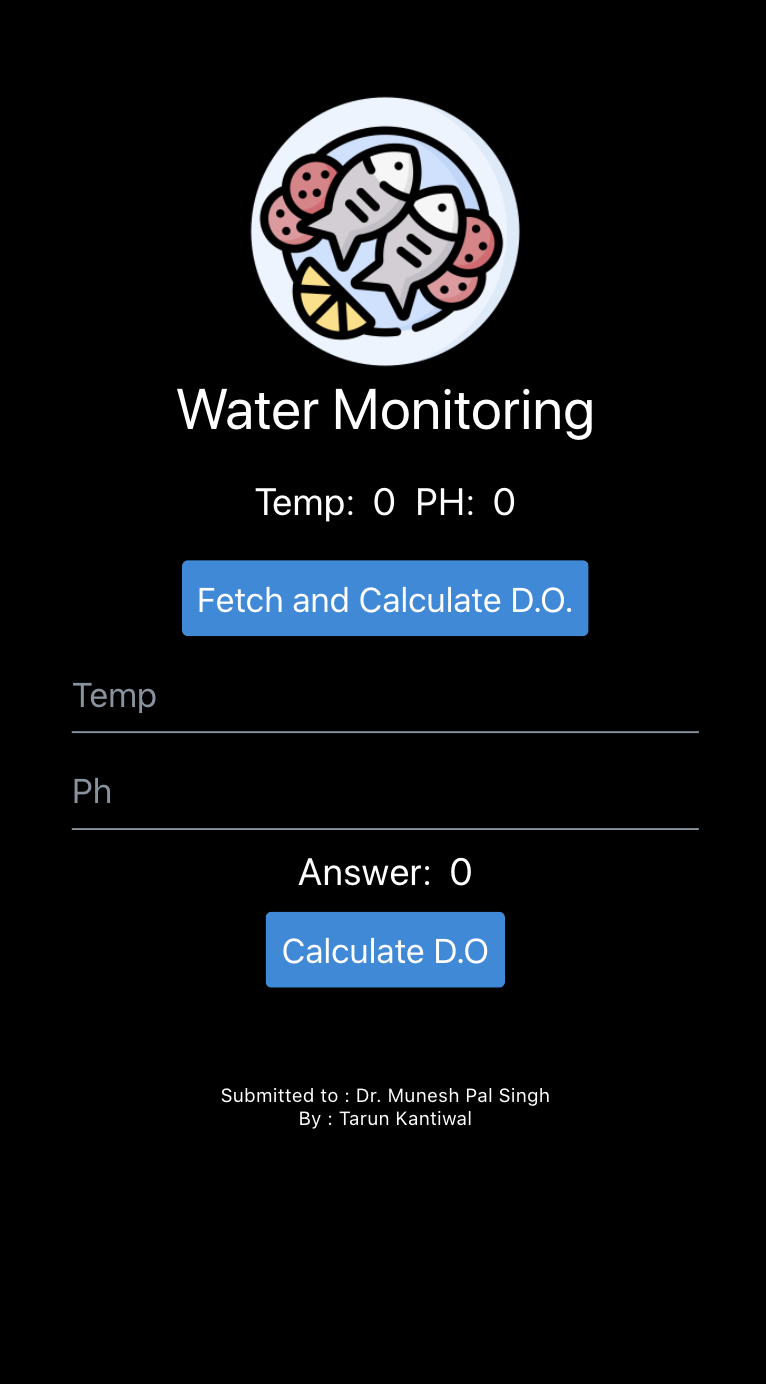
\includegraphics[width=0.6\textwidth]{images/MobileApp.png}\\

By this we completed the mobile Application which we can use in our mobile to make prediction. Now we have a machine learning power on our palm.

\section{What's next ?}
Now We have both Mobile App and web App are ready to use we have to take care of testing and what are the things we have to now take care of, errors.\\


\includegraphics[width=1\textwidth]{images/reactnative.png}\\
